% ---------------------------------
% Example for using \si command
% ---------------------------------
% In the advance from \si{peta\gls*{FLOPS}} to \si{exa\gls*{FLOPS}} performance the issues of \pne present a major hurdle. The associated challenges are identified and tackled by different entities in various ways.

A programming model forms an abstraction layer that connects user applications and parallel computer architectures, leveraging a programming-support library/runtime. Before the advent of task-based parallel programming models, shared and distributed memory models have been used mainly. However, there is no clear boundary of these models. The model design relies on the development of computing and memory architectures, such as multicore, manycore, NUMA architectures. The following introduces conventional models, then details the principle of task-based parallel models.\\

\begin{figure}[t]
  \centering
  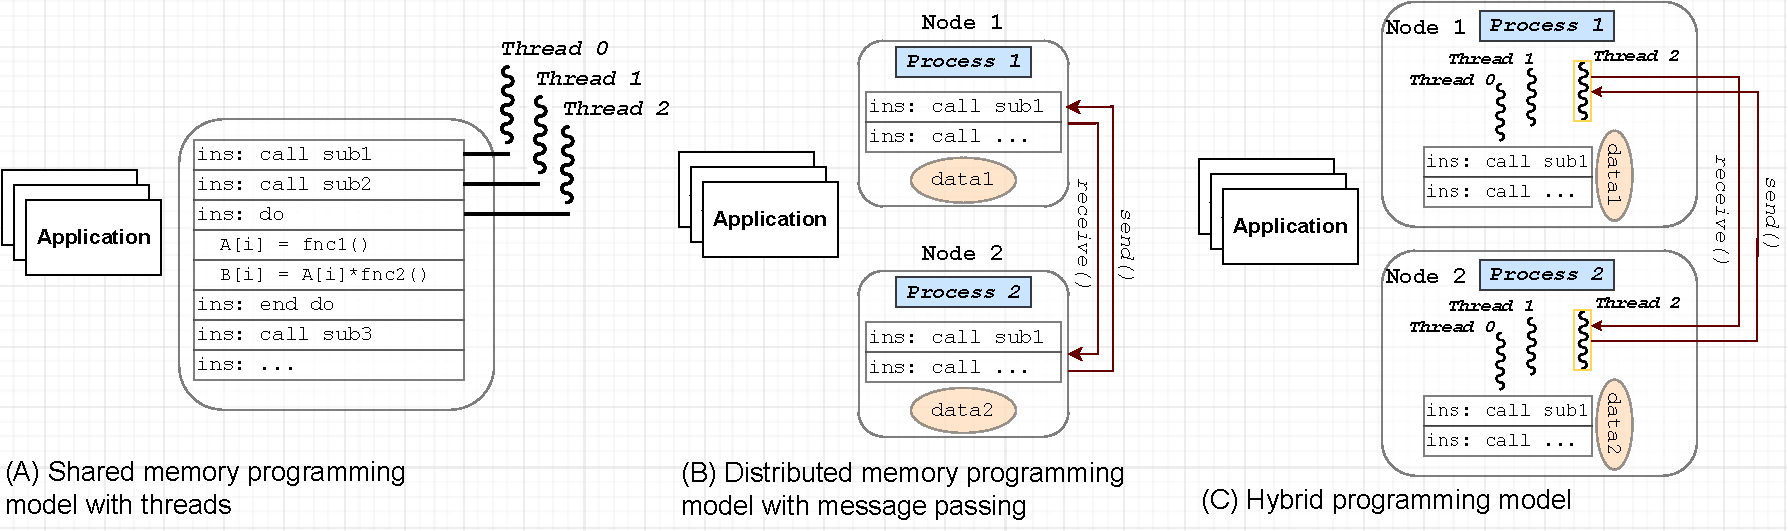
\includegraphics[scale=0.485]{./pictures/preliminaries/preli_conventional_parallel_prog_models.pdf}
	\caption{An overview of shared memory and distributed memory programming models along with their hybrid model.}
	\label{fig:preli_conventional_parallel_prog_models}
\end{figure}

\noindent \textbf{Shared Memory Programming Model}: enables processes or threads to share a common address space. In this model, processes or threads can communicate and synchronize by reading/writing directly from/to shared memory locations. The model allows efficient data sharing. Figure \ref{fig:preli_conventional_parallel_prog_models} (A) illustrates a parallel program using shared memory programming with threads. Here, Thread 0, 1, 2 execute the instructions simultaneously, and the data such as array A and array B are shared. Shared memory programming can be characterized by:
\begin{itemize}
	\item Advantage: simple and straightforward to write programs in parallel. Communication between processes/threads is faster and more efficient than other models requiring inter-process communication.
	\item Disadvantage: difficult to manage data locality. There are challenges in dealing with complex synchronization, race conditions. Incorrect management of shared memory locations can lead to bugs. Furthermore, the scalability might be limited in the scope of a single machine.
	\item Implementation: the most common library is POSIX threads (so-called Pthreads) \cite{butenhof1997programming}. Besides that, OpenMP \cite{dagum1998openmp} is an industry-standard library to support shared memory programming, widely used in various operating systems and compilers. 
\end{itemize}

%\item Threads model: denotes parallel programs using threads. A heavy process can spawn multiple ``lightweight'' threads with concurrent execution paths. Besides POSIX standard, there is another popular API named OpenMP , an industry standard that is easy to use with directive-based declaration.
%This might be considered as the simplest parallel programming model, but sharing can raise contention problems such as race conditions, deadlocks. Various mechanisms called locks/semaphores are proposed. The model has some characteristics as follows.
%Besides, as mentioned, several implementations working on distributed memory machines can also work with shared memory, for example, SHMEM \cite{chapman2010introducing}. Therefore, people often refer to shared memory with or without threads.

\noindent \textbf{Distributed Memory Programming Model}: does not have a shared address space. Distributed memory in this thesis points to physically distributed memory systems where compute nodes connect to each other via a network. Note that memory architectures can also be called distributed in a single machine with NUMA architecture. However, it just appears as distributed memory from the programming view. We demonstrate a distributed memory programming example in Figure \ref{fig:preli_conventional_parallel_prog_models} (B), assuming we have two compute nodes, each creates a process to execute parallel application. The only way to exchange information across these nodes is message passing. For example, Process 2 sends a message to Process 1 and vice versa. Distributed programming models can be characterized by:
\begin{itemize}
	\item Advantage: data and information are exchanged explicitly by sending and receiving messages. Programmers can coordinate nodes to execute tasks and share data on large problems. The scalability of this model is well-suited for HPC and large-scale parallel applications.
	\item Disadvantage: communication overhead is challenging in data decomposition and combination. The problem in a distributed memory model is divided into smaller parts, which are distributed over nodes. After execution, their results and required data need to be combined, which may take time and overhead. Load balancing is also a challenge when task distribution is irrelevant to the system performance model.
	\item Implementation: the most popular library is based on the Message Passing Interface (MPI) standard \cite{gropp1996mpich}. MPI supports API and subroutines that users can define data exchange communication explicitly or implicitly. Besides, several libraries that support message passing at higher levels can also be characterized as distributed memory programming models known as Partitioned Global Address Space (PGAS) \cite{dewael2015pgasl}. PGAS provides an abstraction layer for programmers. We may not need to define the communication of data exchange explicitly. In this thesis, we classify the programming models like PGAS as data-parallel programming models.
\end{itemize}

\noindent \textbf{Data Parallel Programming Model}: refers to Partitioned Global Address Space (PGAS) \cite{dewael2015pgasl}. The idea is to achieve a higher level of abstraction from a programmers perspective. Even on shared or distributed memory, it treats address space globally. For example, the global data structure can be split up logically across tasks in distributed memory systems. Data parallel programming can be characterized by:
\begin{itemize}
	\item Advantage: user-friendly from the programming point of view. The model shows considerable benefits on regular data structures like arrays or matrices.
	\item Disadvantage: in some use cases with complicated data structures, this model cannot ensure performance as well as portability, such as data locality references, the distribution of sparse and irregular data objects. These are important issues for evaluating the efficiency of data-parallel programming models.
	\item Implementation: several implementations such as Coarray Fortran \cite{mellor2009new}, UPC \cite{zheng2014upc}, X10 \cite{chrles2005x10}, Chapel \cite{chamberlain2007chapel}.
\end{itemize}

\noindent \textbf{Hybrid Programming Model}: refers to combining more than one programming model. We have mentioned the hybrid model of shared memory and distributed memory programming, such as MPI+X or MPI+OpenMP \cite{rabenseifner2009hybrid} in Chapter \ref{ch:Introduction}. Shared memory programming models such as OpenMP allow users to specify shared memory locations and threads, but the scalability is limited in a single node. Distributed memory programming models such as MPI allow users to specify communication patterns and processes across nodes. A MPI process is denoted as MPI rank. In MPI-based applications, message passing can occur inside a node when we fully create the number of MPI ranks corresponding to the number of cores. Therefore, the hybrid model exploits benefits from both shared memory and distributed memory programming, such as reducing unnecessary MPI communication inside a node, overlapping communication and computation. Technically, a multicore processor within a node only needs to create one MPI process, where this process can spawn multiple threads. One or a few threads take care of MPI communication while the others execute computation tasks. With the trend of heterogenous computing architectures today, this model is the most relevant. Heterogeneous computing architectures are then implemented as CPUs accelerated by graphics processing unit (GPU) architectures \cite{zhang2011gpumodel}, which are widely used in today's HPC clusters and supercomputers \cite{top500list}. Generally, hybrid models can be characterized by:
\begin{itemize}
	\item Advantage: enables overlapping communication and computation and dealing with data locality. This can be applied similarly for CPU-GPU applications in distributed memory systems, where one or a few threads control communication across nodes, the other threads control computation tasks run on CPU or offloaded to GPU.
	\item Disadvantage: traditional parallel applications need to be changed following the hybrid model. This might lead to conflicts if support libraries or frameworks cannot control the mix of multiple processes along with multiple threads. Furthermore, the hybrid programming model such as MPI+OpenMP might also require users' effort to change conventional applications with pure MPI or pure OpenMP.
	\item Implementation: MPI+OpenMP as an example. Besides OpenMP, MPI can also combine with Pthreads for supporting multithreading inside a process.
\end{itemize}

Figure \ref{fig:preli_conventional_parallel_prog_models} (C) shows an example of a hybrid MPI+OpenMP programming model. The illustrated application is executing on two compute nodes ($Node\ 1$ and $Node\ 2$). Each node deploys an MPI process, $Process\ 1$ belonging to $Node\ 1$ and $Process\ 2$ belonging to $Node\ 2$. Each process spawns three OpenMP threads, where $Thread\ 0$ and $Thread\ 1$ execute the main computation parts, while $Thread\ 2$ is dedicated to performing communication.\\

\begin{figure}[t]
  \centering
  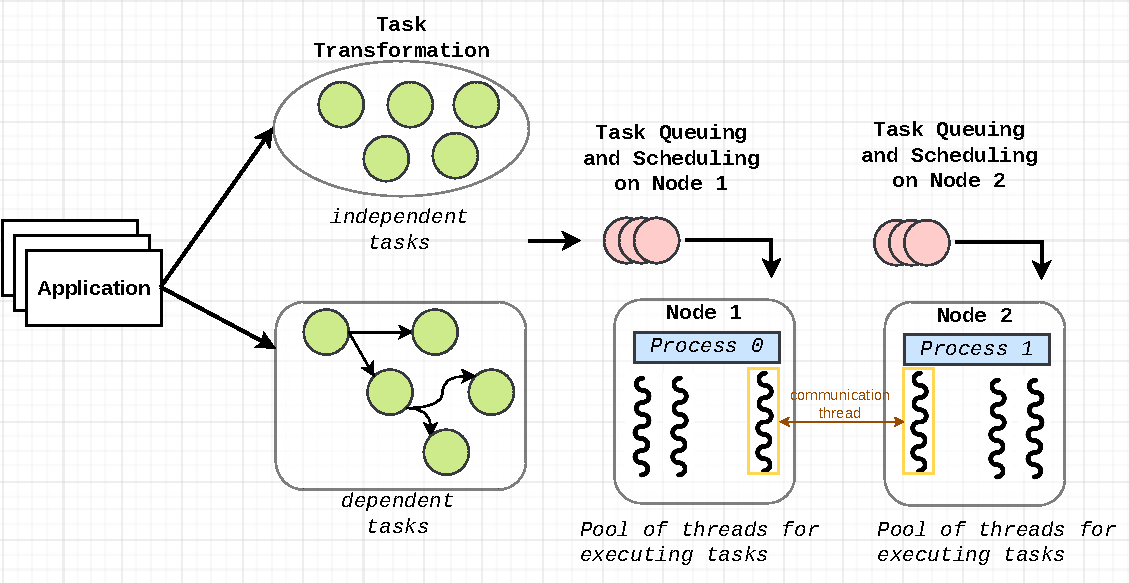
\includegraphics[scale=0.65]{./pictures/preliminaries/preli_task-based_prog_model.pdf}
	\caption{An overview of task-based parallel programming model.}
	\label{fig:preli_taskbased_programming_model}
\end{figure}

\noindent \textbf{Task-based Parallel Programming Model}: is a higher abstraction model based on the hybrid programming model. With the previous programming models in general as well as the hybrid model in specific, it is difficult to manage concurrency issues effectively. Furthermore, today's perspective of low-level programming, such as better performance by tightly controlling hardware, has been changed because users have to make an effort to optimize code among computation, communication, and synchronization. For example, synchronization barriers are often declared in shared and distributed memory programming models and require the user's responsibility. This can lead to performance issues, e.g., causing much idle or waiting time, if we do not control the synchronization tightly.\\

Task-based parallel programming models focus on the criteria of user-friendly coding, portability, and well-expressing parallelism.
The idea of task-based models is to separate the part of tasks, that need to be computed, from the part of computing resources in parallel execution. Users can reduce the burden of controlling how tasks are executed, synchronized, or parallelized. Instead, we just need to define what tasks are, their relationship, and whether they are dependent or independent. Dependent tasks can be represented as a graph of tasks, which is a so-called task graph. An interesting case study formulated as a task graph is game engine \cite{regragui2022schedgameengine}, which is studied to explore task scheduling by Regragui et al.\\

Figure \ref{fig:preli_taskbased_programming_model} illustrates an example of task-based parallel programming. From left to right, the application is assumed to be transformed into a set of tasks. Task transformation depends on how we define a task. A task often points to a compute code entry and its data. The way of transforming tasks or porting normal applications into task-based applications is called tasking. In Figure \ref{fig:preli_taskbased_programming_model}, we assume two cases of task transformation: independent and dependent. The dependent tasks can be addressed as a graph. The next step is queuing and scheduling tasks. Assume we have two compute nodes, $Node\ 1$ and $Node\ 2$. Tasks assigned to $Node\ 1$ are queued and scheduled for execution on $Node\ 1$. Similarly, tasks assigned to $Node\ 2$ are queued and scheduled for execution on $Node\ 2$. Following this, executing tasks on each node is controlled by the task-based programming model, which is usually implemented as a library or framework. During execution, the task-based programming model controls mapping tasks to threads for computation; thus, a task-based model is also called a task-based runtime. After computation, the application's working flow is returned to users.\\

In Figure \ref{fig:preli_taskbased_programming_model}, the view of computing resources on $Node\ 1$ and $Node\ 2$ is similar to the hybrid model, where each node contains a process, a process spawns a pool of threads for task execution. However, users only need to define tasks and are relaxed in managing parallelization, communication, concurrency, or synchronization. We characterize task-based models as follows.
\begin{itemize}
	\item Advantage: user-friendly to develop parallel applications. We can simplify parallel applications with tasks and task relationships. It can be easier to control synchronization and concurrence.
	\item Disadvantage: porting applications from conventional to task-based models might lead to performance issues. Besides, defining tasks in some specific applications is sometimes difficult.
	\item Implementation: there are more and more libraries or frameworks developed to support task-based parallel programming, such as StarPU \cite{augonnet2011starpu}, OmpSS \cite{duran2011ompss}, HPX \cite{kaiser2014hpx}, Taskflow C++ \cite{huang2020cpp}, etc. They are developed in different languages like C++, Python.
\end{itemize}

The next section will show how task-based parallel runtimes are categorized and how task-based parallel applications are characterized in terms of performance issues.

%The idea of task-based programming is not new, where tasks are represented independently or dependently as a graph of tasks (the so-called task graph). Task graphs have been used to model and optimize parallel execution since the early history of computers \cite{codd1960multiprogram}. However, people applied this to the whole jobs instead of defining small tasks in a single application. 

%For task-based programming models, users can reduce effort by expressing tasks and their dependencies without specifying synchronization and concurrence.
%Today, many libraries or runtimes already support task-based models, such as OpenMP tasking \cite{ayguade2008design}, HPX \cite{kaiser2014hpx}, Charm++ \cite{acun2014parallel}.